\chapter{Fundamental Concepts}
\label{cha:fundamentals}
In this chapter we will lay out the fundamental concepts, that are necessary in order to understand the subsequent chapters.
First, we will explain Stream Processing in \ref{sec:stream-processing}. Afterwards, the concept of the self-adaptive systems will be presented and explained in section \ref{sec:self-adaptive} 
followed by a brief explanation of the MAPE loop in \ref{sub:mape} to conclude this chapter.

    \section{Stream Processing}
    \label{sec:stream-processing}
    In this section, we will split the concept of stream processing into three further components.
    In \ref{sub:sps} we will then define stream processing systems, explain how they work and give examplary fields of application.
    Afterwards, in \ref{sub:dsms} we will move on to the topic of data stream management systems.
    % and finally in \ref{sub:requirements} we talk about some requirements that SPSs should meet.
    
        \subsection{Data Stream Management Systems}
        \label{sub:dsms}
        \ifbool{final}{}{\textbf{\color{green}THIS IS FINAL}
        
        }
        % - Streams not saved to disk (Saving to disk and retrieving has high latency), instead kept in memory (low latency)
        % - Some data might still be archived, however it does not impact performance, as it is done parallel to the streaming processing
        % - Sometimes access to archived data in DBMS needed, however this can be cached or efficiently accessed

        \begin{figure}[h]
            
            \centering
            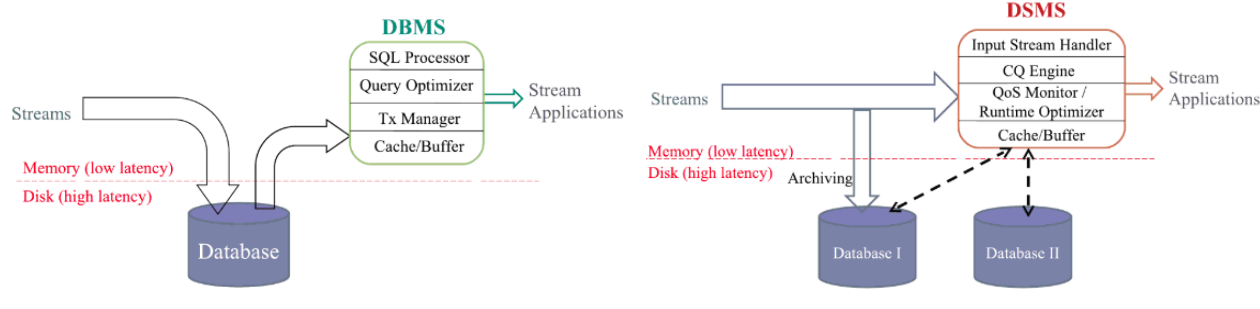
\includegraphics[width=1.0\textwidth]{Bilder/dbms_dsms.png}
            \caption{
                   left: architecture of a DBMS; right: architecture of a DSMS
            }
            \label{fig:dbms_dsms}
        \end{figure}

        A data stream management system is a tool designed to manage continuous data streams.
        DSMSs are comparable to DBMSs, however, there are differences one must take note of.

        \quad Most notably the data being fed into a DSMS varies greatly from the data being inserted into a DBMS. While a DBMS receives a finite predetermined amount 
        of data, a DSMS can theoretically receive an infinite continuous stream.
        % \\
        Secondly, DSMSs operate at a much greater speed than traditional DBMSs, because the data is processed immediately, while in the DBMS approach
        data is first saved to a disk and then queried before further processing can occur, leading to two I/O actions. This behavior, coupled with an incoming 
        high velocity stream, might lead to lags or even failure to yield accurate results \cite{StreamBookQuality}. 
        However, a DSMS might want to archive certain elements from the stream. For this, there are two possibilities:
        Either data is cached in memory, yielding much faster query results, or it is archived in additional databases parallel to the streaming process.
        Thus, the DSMS architecture is superior to the DBMS architecture when it comes to measuring latency.
        When data is stored, oftentimes only synopses are stored, in an attempt to summarize the data and utilize that knowledge in form of a \gls{state} for the queries.
        The difference between these architectures is also shown in figure \ref{fig:dbms_dsms} \cite{StreamBookQuality}.
        % \\
        Lastly, similar to a DBMS, a DSMS can also be queried using a streaming query language. However, queries installed on a DSMS are continuous 
        and will be executed as long as they are not uninstalled and there are restrictions concerning the executability of operations.
        Since the system can not assume a finite amount of data, it processes each data item as it arrives. Meaning that operators that require the entirety of a data 
        set, i.e. the \textit{join} or \textit{aggregation} operators, prove to be problematic when it comes to streams, 
        as they can only return a result once the stream has ended \cite[p.12]{StreamBookQuality}.
        These queries are referred to as \textit{blocking} queries. In order to use them, one must convert them into non-blocking queries.
        One solution for this has been introduced in the form of windows, which are explained in \ref{sub:sps}.

        \quad There are a few more functional differences, which Panigati, Schreiber and Zaniolo highlight, as shown in table 2.1.

        \begin{table}[h]
            \centering
            \label{tab:dbms-dsms}
            \begin{tabular}{|c|c|c|} \hline
                \textbf{Feature} & \textbf{DBMS} & \textbf{DSMS} \\ \hline
                Model & Persistent data & Transient Data \\ \hline
                Table & Set or bag of tuples & Infinite sequence of tuples \\ \hline
                Updates & All & Append only \\ \hline
                Queries & Transient & Persistent \\ \hline
                Query answers & Exact & Often approximate \\ \hline
                Query evaluation & Blocking and non-blocking & Non-blocking \\ \hline
                Operators & Fixed & Adaptive \\ \hline
                Data processing & Synchronous & Asynchronous \\ \hline
                Concurrency overhead  & High & Low \\ \hline
            \end{tabular}
            \captionbelow{Functional comparison of DBMS and DSMS \cite{Panigati2015}} 
        \end{table}

        \subsection{Stream Processing Systems}
        \label{sub:sps}
        \ifbool{final}{}{\textbf{\color{red}THIS IS 90\% FINAL}
        
        }
        % TODO Erklärung von Windows irgendwie einbringen (Hier noch überlegen wo am besten)
        % TODO Challenges, die SPSs facen

        % Topical sentence
        In this section, we will define stream processing systems, expound what data looks like in SPSs. We will also explain what SPSs
        are capable of and give an example of an SPS. Furthermore, windows will be explained and the concept of adaptation in SPSs will be laid out.
        At the end of the section, we will present some of the challenges that SPSs face.

        \quad Stream processing systems are systems designed to handle large amounts of data in (near) real-time fashion with low latency.
        SPSs were designed in order to fulfill the needs for fast processing, which was not solved by the previous batch processing systems.
        Batch processing systems were able to process huge amounts of data as well. However, the difference, that needs to be emphasized, lies in the latency.
        Stream processing systems complete their tasks faster by processing each element as it arrives, as opposed to the batch system, which collects elements 
        and then processes the data in batches.
        The data is fed to the system in form of streams, which are defined as a potentially infinite, countable amount of \textit{data tuples}. 
        The streams usually originate from a \texit{data source} which, for example, can be a type of sensor, e.g. a simple temperature sensor or more complex sensors, 
        such as an EEG-sensor, market orders or network traffic.
        % \\
        A data tuple is an object whose internal structure is defined by a \texit{data scheme}. 
        Objects of a data stream share a common structure, also called \textit{stream schema}.
        Tuples consist of a set of typed attributes and their respective values. One can imagine a tuple as a java object without any operations \cite{fundamentals}.
        Each individual data tuple is processed by one or more \textit{operators}.
        An operator is fed tuples from incoming streams through its input port, performs an operation and generates an output stream through its output port, 
        consisting of the processed tuples. Operators are able to perform various different operations, 
        as shown in \cite[p. 49]{fundamentals}, some of which include: aggregation, splitting and merging streams, 
        logical and mathematical operations and custom data manipulations.
        % \\
        The results of a streaming application are then fed into one or multiple \textit{data sinks}, which could, for example, be a data visualization engine 
        or an automated stock trading engine.
        
        \quad In order for an SPS to perform as fast as possible, it should have the ability to adapt to situations.
        There are many strategies of adaptation, which can be divided into three subcategories: \textit{processing-}, \textit{data-} and 
        \textit{resource adaptation} \cite[p. 8 f.]{QIN20191}. 
        An exemplary resource adaptation would be a \textit{processing scaling} adaptation, as shown in figure \ref{fig:sps_parallel_normal}, 
        where, if computational resources allow it, an operator can be replicated in order to process data faster by
        making use of the principle of parallelity. Technically, there should be a splitting operator placed before the replicated operator, 
        as well as a merging operator after the replicated operator. These have been left out for the sake of brevity.
        % \\
        An example for data adaptation would be \textit{load shedding}, a strategy in which some data tuples are dropped in order to free up computational resources.
        However, one must take into consideration that one possibly sacrifices accuracy for the sake of performance, as more data generally leads to more accurate results.
        Furthermore, one must take note of the resource cost that is needed to calculate which tuples to drop, in order to have the lowest impact on the quality of service.
        % \\
        For resource adaptation we will look at \textit{dynamic resource allocation}. Dynamic resource allocation is a strategy, in which the available computational 
        resources are constantly reassigned, to allocate the memory in the most efficient way possible. For example, a node facing a high data load at the moment can 
        be allocated more RAM, GPU, or CPU power in order to process its load faster. For this to work, some resources have to be freed first, e.g. by deducting some
        computational power from a node facing less input at the time. With this strategy, one must take into consideration the resources and time spent calculating 
        the optimal allocation of resources.

        % Challenges
        \quad By nature of the fields in which stream processing is applied, SPSs face a series of challenges.
        
        \quad As SPSs are used as a means to process big data in a (near) real-time fashion, we will take a system that predicts changes in stock values 
        of companies based on the public's opinion, which is extracted from tweets, as an examplary application.
        % \\
        The application receives new \gls{tweet}s as input, then performs operations such as clustering and filtering for certain terms or company names. 
        Afterwards, a sentiment analysis is performed on said tweets and a prediction for stock prices is computed and then sent 
        to an automatic stock trading application and stock traders for manual reviews.


        \begin{figure}[h]
            \centering
            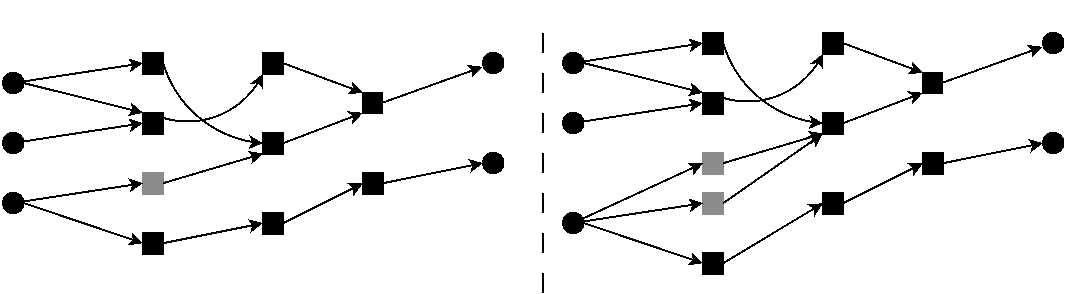
\includegraphics[width=1.0\textwidth]{Bilder/sps_parallel_normal.png}
            \caption{
                    left: An example for an SPS displayed as a directed acyclic graph;
                    right: Same SPS with introduced parallelity in one operator, also called scale-out adaptation, marked gray for visibility;
                    Circles on the left depict data sources, circles on the right depict data sinks, squares are operators/processors, and arrows are streams.
            }
            \label{fig:sps_parallel_normal}
        \end{figure}

        % Subsection Requirements for Stream Processing Systems
        % Should quickly go over the requirements and explain why they matter to us
        % \subsection{Requirements for Stream Processing Systems}
        % \label{sub:requirements}
        % \ifbool{final}{}{\textbf{\color{red}THIS IS NOT FINAL}
        
        % }

        % Notes: What are the requirements, why do they matter to us (Elaborate on this)

        % Due to the nature of the fields in which SPS are used, there are important requirements that SPS should meet in order to be viable, 
        % which Stonebraker et al. point out in \cite{Stonebraker:2005:RRS:1107499.1107504}, of which the ones most important to us can be summarized as the following:
        
        % % Enumeration of requirements for SPS + explanations why they matter to us
        % \begin{enumerate}
        % \label{enum:requirements}
        %     \item \textbf{Keep the Data Moving:} 
        %         In order to minimize latency, data must not be stored, as these are costly operations.
        %     \item \textbf{Handle Stream Imperfections:} 
        %         Expecting only perfect data is utopian, so one must prepare the system with built-in mechanisms for data that might be missing or out-of-order.
        %     \item \textbf{Integrate Stored and Streaming Data:} 
        %         For an SPS to be able to perform comparisons between "predecessor" data and current data, operators must keep an efficiently manageable state.
        %     \item \textbf{Guarantee Data Safety and Availability:} 
        %         Recovering from a failure is detrimental for real-time data processing, so a system must be in place to guarantee the highest availability possible.
        %     \item \textbf{Process and Respond Instantaneously:} 
        %         Systems must be highly optimized in order to provide (near) real-time responses.
        %     \item \textbf{Partition and Scale Applications Automatically:} 
        %         Systems must be able to be split across multiple machines and threads.
        %         The system must also be able to automatically scale and distribute the load across the machines.

        % \end{enumerate}

    \section{Self-Adaptive Systems}
    \label{sec:self-adaptive}
    \ifbool{final}{}{\textbf{\color{green}THIS IS FINAL}
    
    }{}
    
    Cheng et al. define self-adaptive systems as
    \begin{quotation}
        ``[\ldots] systems that are able to adjust their behaviour in response to their perception of the environment and the
        system itself [\ldots]``\cite[p. 1]{Cheng:2009:SES:1573856.1573858}.
    \end{quotation}
    
    \quad Self-adaptive systems are oftentimes based on the \nameref{sub:mape} pattern.
    Adaptive systems have a wide variety of possible application areas: adaptable user interfaces, autonomic computing, multi-agent systems \cite{Cheng:2009:SES:1573856.1573858}, 
    biologically inspired computing, robotics \cite{10.1007/978-3-319-59480-4_44}, streaming applications, etc.

    \quad An example for an application would be a scenario, in which population and food capacities are given and evolving over time, due to births, deaths, changes in demographics, 
    and changes in weather and harvest respectively. A system would have to adapt to these changes in its environment in order to ration the food properly.

    \quad Self-adaptivity however presents itself as challenging when looked at from a software engineering perspective.
    Cheng et al. illustrate some of these challenges in \cite{Cheng:2009:SES:1573856.1573858}, which we will discuss in the following paragraphs for both the 
    requirements engineering and the architecture disciplines.
    % \\
    As the system adapts, it changes, and with it, do the requirements. This leads to the fact, that language changes in requirements engineering.
    Usually, requirements are formulated in a strict manner `\textit{The system shall\ldots}`. This has to be relaxed and changed, Cheng et al. propose the following 
    option amongst others: `\textit{The system may do this\ldots or it may do that\ldots}`.
    % \\
    More importantly, requirements engineering must define exactly what is monitored, as well as high-level goals, which need to be fulfilled under any given environmental condition.
    In addition, one must also specify under which circumstance the kind of adaptation that has to be performed and how said adaptation is realized.
    Due to the increased amount of requirements and the everchanging nature of an adaptive system, it gets harder to trace whether requirements are fulfilled, which adds to the complexity.
    % \\
    One must also take into account that it is nearly impossible to forecast every situation that a system may face. 
    This incomplete information adds to the challenges that requirement engineers are facing.

    \quad The complexity is also increased for engineers and architects, as there are new factors to consider as well.
    Single MAPE loops do not scale efficiently for large systems, one must find a better scaling solution. Often times multiple control loops are constructed.
    Good practice, however, suggests using just a single control loop \cite{accidents}, which means that one should try to minimize the amount of control loops used and
    make them independent from one another.
    
    
    \quad Architects are faced with a number of new decisions;
    % \\
    Is a centralized or decentralized architecture better for achieving one's goals? Are the control loops independent from one another?
    Is a hierarchical approach appropriate? Can the amount of control loops be scaled down?
    % \\
    Research is needed to battle some of the issues that self-adaptive systems and control structures face, such as structural arrangements. 
    It is therefore necessary to explore more architectures, an example for which will be shown in \ref{sec:hierarchical}, where a decentralized hierarchical approach was
    chosen to combat said issues. In addition, evolving an existing system into a self-adaptive system currently requires a lot of work. 
    A possible field of research would be finding a way to 'inject' self-adaptivity into pre-existing systems.
    
    \quad Cheng et al. propose that control loops be made explicit and kept seperate so as to 'seperate the concerns of functionality from the concerns of self-adaptation' \cite[p. 16]{Cheng:2009:SES:1573856.1573858}.
    Furthermore, they emphasize the importance of understanding control loops as the most important tool in self-adaptive systems in order to mature the research area of self-adaptive systems.
    
    \subsection{MAPE-K Loop}
    \label{sub:mape}
    \ifbool{final}{}{\textbf{\color{green}THIS IS FINAL)}
    
    }{}
    % Explain the MAPE-K Loop as it is a valuable basis/reference architecture for many different approaches in adaptive systems
    % Rough explanation of what it is, where it is used
    % explain different "stages" (m, a, p, e)
    % Explain -K extension
    The MAPE-K Loop was introduced by IBM \cite{Kephart:2003:VAC:642194.642200} and refers to a proposed solution for self-adaptive or autonomic systems.
    This model, as shown in figure \ref{fig:mape}, has since become the basis or reference architectural pattern for many self adaptive systems, which we will show in the third chapter.
    The acronym \textit{MAPE-K} refers to the components that constitute the model:
    \begin{figure}[hbt]
        \centering
        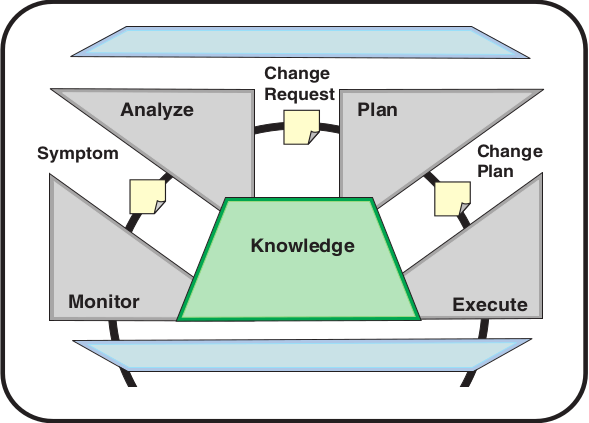
\includegraphics[width=0.45\textwidth]{Bilder/mape.png}
        \caption{
                Overview of the MAPE-K-Loop\cite{Kephart:2003:VAC:642194.642200}
        }
        \label{fig:mape}
    \end{figure}  

    \begin{enumerate}
    \label{enum:mape}
        \item \textbf{M}onitor: 
            The \textit{Monitor} component gathers data about the system and its environment, aggregates, and filters it.
        \item \textbf{A}nalyze: 
            The \textit{Analyze} component analyzes the previously gathered data and determines whether or not an adaptation should be performed.
            The decision is based on performance or cost gain and should include the adaptation cost as well.
            This component's analysis is influenced by the \textit{Knowledge} base.
        \item \textbf{P}lan: 
            If the choice to adapt the system has been made, the \textit{Plan} component then decides how to reconfigure the system.
            Once the decision has been made, the information is then forwarded to the \textit{Execute} component.
        \item \textbf{E}xecute: 
            Given the \textit{Plan} component's decision, the \textit{Execute} component then executes said plan and the loop 
            returns to the initial monitoring state.
        \item \textbf{K}nowledge: 
            Represents the knowledge base, which is shared between the other components.
            This base is created by the \textit{Monitor} component and contains information in the form of metrics, policies, symptoms and logs.
    \end{enumerate}
   


\chapter{Approaches for Self-Adaptive Architectures in Stream Processing}
\label{cha:approaches}
% \textbf{TODO: How does it work? FOCUS ON ARCHITECTURE IN THIS CHAPTER!!}
In this chapter, we will showcase two approaches for self-adapting stream processing systems.
In \ref{sec:dhalion} we will present Dhalion, a system that sits on top of streaming engines, such as Heron, and allows them to become self-regulating, as described in \cite{dhalion}.
Furthermore, we will give an outline of Heron in \ref{sub:heron-outline} and then explain Dhalion's architecture in detail in \ref{sub:dhalion-architecture} which we then discuss in \ref{sub:dhalion-discussion}.
In \ref{sec:hierarchical} we will explore a decentralized hierarchical approach to self-adaptive stream processing systems, as proposed in \cite{cardellini}. Analogous to the \nameref{sec:dhalion} chapter, we will first 
explain the proposed architecture in \ref{sub:edf} and follow it up with a discussion in \ref{sub:discussion-edf}.

    \section{Dhalion}
    \label{sec:dhalion}
    Dhalion is a framework developed by Floratou et al., which is used on top of streaming engines, giving said underlying systems the ability to self-regulate.  
    Floratou et al. define three characteristics that a self-regulating system has to be capable of:
    
    \quad \textit{Self-tuning}: A self-regulating system should be self-tuning, meaning that a self-regulating system should 
    be able to take both the policy, which defines the objective, and the specification of the streaming system and automatically tune 
    its configuration parameters in a matter that leads to the fulfilment of its service level objectives.
    
    \quad \textit{Self-stabilization}: As the rate of incoming streams fluctuates, a system can be faced with either over- or under-utilization of its computing resources. 
    In order to prevent these issues, a self-regulating system has to react to changes in the stream velocity and either acquire additional resources 
    or free resources and scale down.

    \quad \textit{Self-healing}: Due to the fact that systems can not only be affected by failures but also by reduced quality of service, 
    e.g. a slow disk or memory constraints, self-regulating systems need to have a mechanism in place to diagnose such service degradations and to adapt 
    to recover from such faults.

    In order to get a deeper understanding of Dhalion, we will briefly explain Heron in \ref{sub:heron-outline}, then discuss Dhalion's architecture in \ref{sub:dhalion-architecture}, 
    which we then follow with a discussion of Dhalion in \ref{sub:dhalion-discussion}.

        \subsection{An Outline of Heron}
        \label{sub:heron-outline}
        Small outline of Heron, as Dhalion is built on top of Twitter's Heron.

        \subsection{Dhalion's Architecture}
        
        \label{sub:dhalion-architecture}
        Dhalion is a modular framework that allows streaming systems to become self-regulating and consists of 3 major components.
        Its architecture is shown in figure \ref{fig:dhalion}.

        \begin{figure}[hbt]
            \centering
            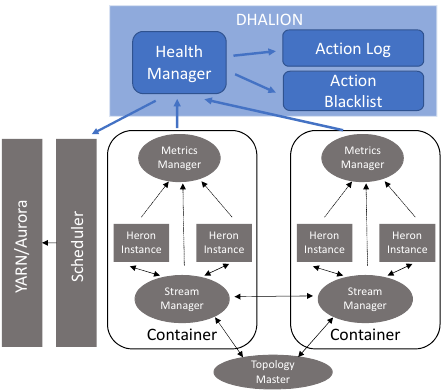
\includegraphics[width=0.5\textwidth]{Bilder/dhalion.png}
            \caption{
                Architecture of Dhalion, sitting on top of Heron. Dhalion components marked blue \cite{dhalion}.
            }
            \label{fig:dhalion}
        \end{figure}

        \quad The biggest component of Dhalion is its \textit{health manager}, who is responsible for maintaining the health of the topology.
        The health manager periodically invokes a policy which evaluates the health of the topology. 
        The policies used by the health manager can either be noninvasive or invasive, meaning that they can either only alert the user when a particular event occurs or 
        perform certain adjustments to the topology's configuration, respectively.
        Its possible to execute multiple noninvasive policies at a time, however, one can only execute one invasive policy at a time.
        The health manager works in 3 phases: the \textit{symptom detection phase}, the \textit{diagnosis generation phase} and the \textit{resolution phase}.
        
        \quad During its first phase, the symptom detection phase, Dhalion collects several metrics, which are then used to identify symptoms, that could indicate that the 
        topology's health is in jeopardy.
        This identification process is performed by \textit{symptom detectors}, which collect appropriate metrics and form evaluations based on the collected metrics.
        Symptom detectors employ multiple forms of anomaly detection techniques, such as outlier detection and clustering.
        Once a sympton has been identified by a symptom detector, a symptom description will be generated. A symptom description contains the sympton, the metrics which
        were used to identify the symptom, and the corresponding values of those metrics.
        Additionally, Dhalion's extensive API offers end-users the ability to design their own symptom detectors.
        
        \quad In the diagnosis generation phase, the health manager collects the symptoms generated during the symptom detection phase and attemps to identify the causes 
        of the symptoms. 
        This is done via diagnosers. Diagnosers take a set of symptom descriptions as input and output a diagnosis description based on the symptons. 
        A diagnosis description contains the cause, the corresponding symptoms as well as the metrics and their values that led to the diagnosis.
        Similarly to the symptom detectors, end-users are able to create their own diagnosers via Dhalion's API.

        \quad During the health managers final phase, the resolution phase, it attempts to resolve the previously diagnosed problems.
        Resolvers, who perform the resolving process, process the diagnoses descriptions provided by the diagnosers and perform the 
        appropriate actions, based on the diagnoses, to improve the topology's health. Usually, there is a 1:1 mapping between resolvers and diagnosers.
        First, the system determines the appropriate resolver by examining the diagnoses. Afterwards, the designated resolver performs the topology changes.
        However, major topology changes, such as scaling up/down or restarting containers, are invoked through the scheduler, as shown in figure \ref{fig:dhalion}.
        The Dhalion API offers end-users the possibility to create their own reolvers.

        \quad The system's second component is the \textit{action log}, which records the actions taken by the health manager.
        The log can be useful for tuning or debugging policies. Each entry consists of the action that was taken, the time at which the action took place and the diagnosis 
        that led to the action being executed. 
        It is noteworthy that the end-users can configure Dhalion to drop logs once they pass a certain size or age.

        \quad The system's third and final component is the \textit{action blacklist}, which end-users have the ability to not use for policies.
        After each action, the health manager waits until the topology has once again reached a steady state and then evaluate the performed action.
        To do this, one must define an evaluation method whenever one creates a new policy. Given the evaluation method, the health manager evaluates the action.
        If the action does not reach the desired results, and the amount of times it was beneficial to the topology's health divided by the total amount of times it 
        was invoked passes a pre-defined threshold, the action will be blacklisted.
        Before a resolver can invoke a certain action, it must first check the blacklist to see if this action has been blacklisted for a similar diagnosis.

        \subsection{Discussion of Dhalion}
        \label{sub:dhalion-discussion}
        Due to Dhalion's extensive API end-users are able to create their own policies and thus expand Dhalion to fulfill their needs. 
        The modularity offered by Dhalion's policy architecture allows for the creation of many different objects, e.g. diagnosers, resolvers or symptom detectors, 
        instead of having to create monolithic objects.
        This approach promotes reusability of e.g. diagnosers for multiple policies and allows for easier debugging and evaluation.
        Furthermore, existing code is much easier to be maintain, as one does not have to understand a monolithic structure but instead only smaller objects.
        
        \quad However, if some fault occurs during the settling resting period, after which an action is evaluated by the health manager, occurs, Dhalion has no means to 
        identify what caused the problem and might erroneously blacklist an action that might have been beneficial.

        \quad The approach that Floratou et al. took can be compared to be MAPE loop. The monitor phase is being performed by the health manager's symptom detector, who collects metrics.
        The analysis phase is done by the symptom detector, who analyzes the metrics and identifies symptons, as well as the diagnoser, who forms diagnoses.
        The planning and execution phases are completed by the resolver, who determines the necessary action and then executes it.

    \section{Decentralized Self-Adaptation}
    \label{sec:hierarchical}
    In this section we will explore a decentralized hierarchical architecture as described by Cardellini et al in \cite{cardellini}.
    % \\
    In \ref{sub:edf} we will present the proposed architecture, as shown in figure \ref{fig:hierarchical}, and elaborate on its functionality in greater detail.
    % \\
    Afterwards we will discuss the architecture, talk about the advantages and possible complications. Further we will compare it to its reference architecture in \ref{sub:discussion-edf}.


        \subsection{Elastic and Distributed DSP Framework}
        \label{sub:edf}
        As previously mentioned, a single MAPE loop often poses as a threat to become a bottleneck and does not scale well in larger systems\cite{cardellini}\cite{Cheng:2009:SES:1573856.1573858},
        Cardellini et al. argue to implement multiple MAPE loops, as per Weyns et al. \cite{Weyns2013}, which are organized in a hierarchical pattern to achieve decentralized control.
        % \\
        \begin{figure}[hbt]
            \centering
            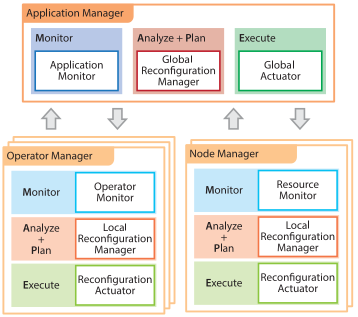
\includegraphics[width=0.5\textwidth]{Bilder/hierarchical.png}
            \caption{
                    Conceptual architecture of the EDF\cite{cardellini}
            }
            \label{fig:hierarchical}
        \end{figure}
        The proposed architecture makes use of two different abstraction layers, allowing a separation of concerns. 
        While the higher abstraction layer works on a slower time scale, the lower abstraction layer works on a faster time scale.
        % \\
        The MAPE loops are arranged in a hierarchical pattern, where higher-level loops are in charge of the decisions proposed by the lower-level loops.
        % \\
        On the lower layer Cardellini et al. introduce two new concepts; the \textit{operator manager} and the \textit{node manager}.

        \quad The operator manager is in charge of controlling the adaptation of a single operator by utilizing a local MAPE loop.
        The architecture utilizes as many operator managers as there are operators.
        The operator manager consists of three further concepts;
        % \\
        The \textit{operator monitor}, which is responsible for the monitoring the resource usage and performance of the operator.
        % \\
        The \textit{local reconfiguration manager}, which manages the analysis and planning phase of the MAPE loop, by first analyzing the collected information 
        from the monitoring component, followed by planning the adaptation, which can either be a scale-in our scale-out, 
        as shown in figure \ref{fig:sps_parallel_normal} adaptation for the operator.
        Once the local reconfiguration manager has decided that a local adaptation is appropriate it will file an operator adaptation request to the higher layer.
        % \\
        If the higher level control structur deems the reconfiguration request reasonable, it will notify the lower level's \textit{reconfiguration actuator}, which will then 
        perform the scaling-in or -out operation.

        \quad The node manager is an entity that manages a single node, whose task it is, to oversee the computing environment of said node.
        There are as many node managers as there are nodes.
        Its ultimate goal is to prevent overuse of available resources.
        Similar to the operator manager it utilizes a singular local MAPE loop to control the adaptation, 
        which can be a migration of a hosted replicated operator to a neighboring node. 
        % \\
        Analogous to the operator manager, it also consists of three further components;
        % \\
        The monitoring component of the operator manager's loop is handled by the \textit{resource monitor}, which collects data about the node's resource usage.
        The collected data is then passed to the \textit{local reconfiguration manager}, which, similarly to the operator manager's local reconfiguration manager, then
        analyzes the data and, if need be, plans a migration. 
        % \\
        Once a decision has been made by the local reconfiguration manager, it then sends a request to the higher layer. Analogous to the operator manager, the \textit{reconfiguration actuator} will perform
        the adaptation if the higher layer authorizes the reconfiguration.

        \quad The higher layer contains a singular \textit{application manager} instance, which contains a global MAPE loop.
        The application manager functions as a centralized entity, whose goal it is, to oversee the entire application through its loop.
        Similar to the lower layer's operator and node managers, it is also split up into three components;
        % \\
        The \textit{application monitor}, which supervises the application behavior on a global scale and collects data, which then gets sent to the \textit{global reconfiguration manager}.
        The global reconfiguration manager is more complex than the local reconfiguration managers of the lower layer entities, as it not only analyzes the collected data, but 
        also analyzes the reconfiguration requests from the lower layers. After the analysis, possible adaptations are planned.
        % \\
        Once a decision has been reached, information is passed over to the \textit{global actuator}, who then communicates the decisions to the lower layer's managers, 
        where the respective reconfiguration actuators perform the adaptations.
        
        \quad In order to determine the sequence of the adaptations, Cardellini et al. use a \textit{pause-and-resume approach}\cite{Heinze2014CloudbasedDS}, 
        which implies that the operator, that is to be adapted, will be paused while the adaptation is performed and resume its functionality after the 
        reconfiguration has taken place. 
        % \\
        Furthermore, to remain integrity of the stream while adaptations are made, they make use of the \textit{stateful migration protocol}, 
        which they have proposed in \cite{migrationProtocol}. The protocol states that the operator's state, given that it is a stateful operator, 
        will be saved to persistent memory, e.g. a database. During the reconfiguration any incoming data will be buffered in memory.
        As soon as the adaptation has been performed, the state will be restored and the buffered data will be processed.
        This process, of course, leads to bigger downtime, so it is even more important to very carefully choose, whether an adaptation is made or not.
        To determine when a request for an adaptation should be granted, Cardellini et al. propose policies for the lower layer's managers.
        % \\

        \quad The operator manager policy utilizes the limited view on system, which only lets it access the input rate and the utilization of its operator.
        It implements a local policy, which is responsible for planning the scaling-in and scaling-out actions. Cardellini . propose two different policies.
        The first one is a threshold based policy, which the the most commonly used technique. The threshold is usually based on empiric data. Once the CPU utilization 
        of an operator passes the threshold, a scale-out action will be planned. 
        % \\
        The second approach makes use of reinforcement learning, where ... {TODO nochmal nachlesen}.
        % \\ 

        \quad The node manager policy is in place to avoid over utilization of a node's computing resources. 
        It utilizes its knowledge about the node's CPU utilization and its network distance to neighboring nodes.
        This policy uses a threshold based approach, too. As soon as the CPU utilization passes the threshold, a hosted replica will be selected 
        randomly and then migrated to a neighboring node, which is randomly selected, with closer neighbors being preferred. 

        \quad The application manager policy exploits its centralized position and its global view. 
        Its responsibility lies in resolving resource acquisition conflicts as well as in limiting of reconfigurations, 
        in order to reduce the amount of downtime. Furthermore, it should encourage the local managers to plan reconfigurations when the system 
        is performing poorly. Conversely, when the system is not experiencing any changes in the working environment, it should promote a settling period, 
        in which no reconfigurations should be made.
        The policy works in 3 steps:

        \begin{enumerate}
            \item \textit{reconfiguration request prioritization}, during which the most worthy reconfigurations are determined by sorting the requests 
            by type and reconfiguring score, which is given by the lower layer's decentralized managers. 
            \item \textit{conflict prevention}, which checks for requests that are trying to use the same computing resource. If a conflict is found, the 
            request with the lower reconfiguration is removed.
            \item \textit{acceptance of requests}, where the remaining requests will be approved and the decision sent to their respective managers. 
            One could either accept all remaining requests or somehow reduce the amount of requests further.
        \end{enumerate}
        % TODO - hier koennte man theoretisch noch deren token bucket based granting policy vorschlagen


        \subsection{Discussion of EDF}
        \label{sub:discussion-edf}
        During the development of their EDF Cardellini et al. explored two different architectural patterns: The master-slave pattern and the coordinated control pattern.

        \begin{figure}[hbt]
            \centering
            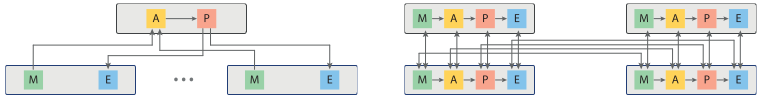
\includegraphics[width=1.0\textwidth]{Bilder/master_coordinated.png}
            \caption{
                    left: master-slave pattern; right: coordinated control pattern\cite{cardellini}
            }
            \label{fig:master_coordinated}
        \end{figure}

        \quad The master-slave pattern has a centralized master component, which executes the analyze and planning phases, and multiple decentralized slave components, 
        who each execute the monitor and execution phases. This pattern is shown on the left in figure \ref{fig:master_coordinated}.
        The master component is in charge of deciding when and how an adaptation should take place.
        Additionally, the master component allows for the creation of a global self-adaptation policies, which are easier to design.
        The centralized component can however still proof to be a bottleneck, especially in a geo-distributed environment, as there might be severe communication overhead, when communicating 
        with the decentralized slave components, as all monitored data as well as all decisions must be transferred to the master component and slave components, respectively. 

        \quad The coordinated control pattern, as shown on the right in figure \ref{fig:master_coordinated}, utilizes multiple decentralized MAPE-loops, who each oversee a certain part of the system. 
        The loops may also needs to coordinate with one another, in case they need to make joint decisions. Again, one must watch out, as to not create too big of an overhead due to too much communication.
        However, one must also ensure that there is enough communication so that there won't be too frequent adaptations, as those may worsen the application's performance.
        Also, due to the decentralization it becomes harder to design control policies.
        
        \quad The final EDF architecture is not too restrictive, so that the end-user can design use other internal policies and goals. 
        One can decide to use a simple threshold based policy for the local policies or sophisticated reinforcement learning policies, which can account for various 
        quality of service metrics. This way, the end-user can decide which metric they want to emphasize on.
        Furthermore, a fully decentralized control solution shows to be very good in terms of performance.
        The reinforcement learning could also be sped up by choosing more sophisticated methods, Cardellini et al. suggest bayesian decision trees and function approximation.

        \quad In addition, Cardellini et al. also consider giving the global policy more influence on the lower level policies by letting the 
        global policy adjust the parameters of the local policies or simply giving more informative feedback rather than just acceptance or denial of the adaptation request.

        % TODO compare it to the reference architecture

    % \section{Title??}
    % \textbf{TODO: Discuss among all of them, critical thinking..}

    % \textbf{TODO: If enough material compare the architecture relevant metrics of the approaches}